%%%%%%%%%%%%%%%%%%%%%%%%%%%%% Define Article %%%%%%%%%%%%%%%%%%%%%%%%%%%%%%%%%%
\documentclass{article}
%%%%%%%%%%%%%%%%%%%%%%%%%%%%%%%%%%%%%%%%%%%%%%%%%%%%%%%%%%%%%%%%%%%%%%%%%%%%%%%

%%%%%%%%%%%%%%%%%%%%%%%%%%%%% Using Packages %%%%%%%%%%%%%%%%%%%%%%%%%%%%%%%%%%
\usepackage{listings, xcolor}
\usepackage{parskip}
\usepackage{hyperref}
\usepackage{amsmath}
\usepackage{graphicx}
\usepackage[a4paper, margin = 1.5cm]{geometry}
\usepackage{float}
\usepackage{amssymb}

%%%%%%%%%%%%%%%%%%%%%%%%%%%%%%% Title & Author %%%%%%%%%%%%%%%%%%%%%%%%%%%%%%%%
\title{Diagramma Classi - Aspetti Avanzati}
\author{Trentin Tommaso}
%%%%%%%%%%%%%%%%%%%%%%%%%%%%%%%%%%%%%%%%%%%%%%%%%%%%%%%%%%%%%%%%%%%%%%%%%%%%%%%

\begin{document}
  \maketitle
  \tableofcontents
  \newpage

  \section{Dipendenze}
    Dependency si rappresentano mediante una linea tratteggiata \textbf{unidirezionale} che termina con una freccia dall'oggetto dipendente (\textit{client}) a quello da cui dipende (\textit{provider}).
    \begin{itemize}
      \item Si ha una dipendenza tra due classi se la modifica della definizione della classe provider può causare cambiamenti nella classe client; 
      \item Se provider viene modificato e cambia la sua interfaccia, tale modifica deve coinvolgere anche il client $\rightarrow$ \textit{effetto domino} per sistemi complessi in caso di modifiche potenzialmente onerose. 
    \end{itemize}
    \subsection{Tipologie di dipendenza}
      Per distinguere tipologia di dipendenza UML mette a disposizione stereotipi, indicati con keywords tra <<>>:
      \begin{itemize}
        \item \textbf{<<use>>}: client effettua generico uso di qualcosa della destinazione (\textit{dipendenza d'uso generica});
        \item \textbf{<<call>>}: client invoca un'operazione del provider;
        \item \textbf{<<create>>}: client crea istanze del provider.
      \end{itemize}
    \subsection{Implicazioni}
      Dipendenze sono individuate solitamente durante progettazione di dettaglio, raramente contribuiscono a modello concettuale:
      \begin{itemize}
        \item Durante testing, correttezza del client è vincolaa a qualla del provider; 
        \item Client non può essere riusato senza provider; 
        \item Modifiche di provider implicano modifiche di client (\textit{ripple effect} - con troppe dipendenze modificare una classe implica modificarne molte altre).
      \end{itemize}
  \section{Interfacce e Classi Astratte}
    \subsection{Classi ed Operazioni Astratte}
      Una classe astratta è una classe che non può essere direttamente istanziata poiché ha \textbf{una o più operazioni astratte} (dichiarate ma non implementate), in UML si rappresenta scrivendo nome in corsivo (o con etichetta {abstract}). 
      \begin{figure}[h!]
        \begin{center}
          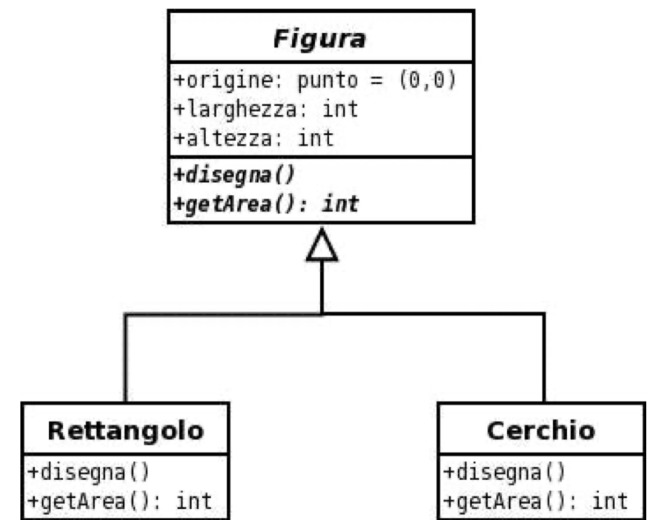
\includegraphics[width=0.5\textwidth]{figures/abs_cl.png}
        \end{center}
      \end{figure}
*
    \subsection{Interfaccia}
      \begin{itemize}
        \item Classe priva di implementazione (\textbf{tutte le operazioni sono astratte}); 
        \item Descrive porzione di comportamento visibile, comune ad un insieme di oggetti; 
        \item Una o più classi possono fornire implementazione dell'interfaccia; 
        \item In UML si usa notazione grafica simile alle classi, ma con keyword \textbf{<<interface>>}; 
        \item Classi che implementano un'interfaccia devono fornire un'implementazione per \textbf{tutti} i metodi dichiarati nell'interfaccia.
      \end{itemize}
      Idea di base è separare specifica di una funzionalità (interfaccia) dall'implementazione della stessa da parte di una o più classi, con due possibili rappresentazioni:
      \begin{figure}[h!]
        \begin{center}
          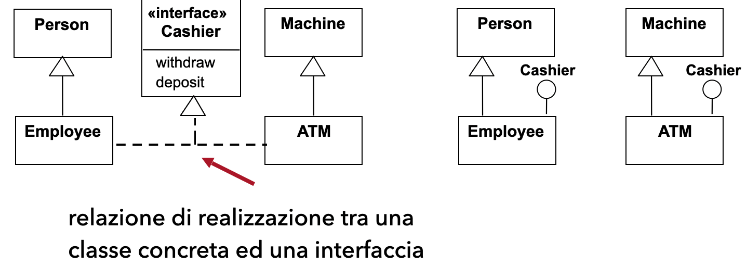
\includegraphics[width=0.5\textwidth]{figures/interface.png}
        \end{center}
      \end{figure}
    \subsection{Classi e Interfacce}
      Classi hanno due tipi di rapporti con interfacce:
      \begin{itemize}
        \item Classe può \textbf{fornire} interfaccia se è sostituibile ad essa (praticamente la implementa); 
        \item Classe può \textbf{richiedere} interfaccia se ha bisogno di una sua istanza per funzionare (forma di dipendenza).
      \end{itemize}
      \subsubsection{Esempio}
        \begin{figure}[h!]
          \begin{center}
            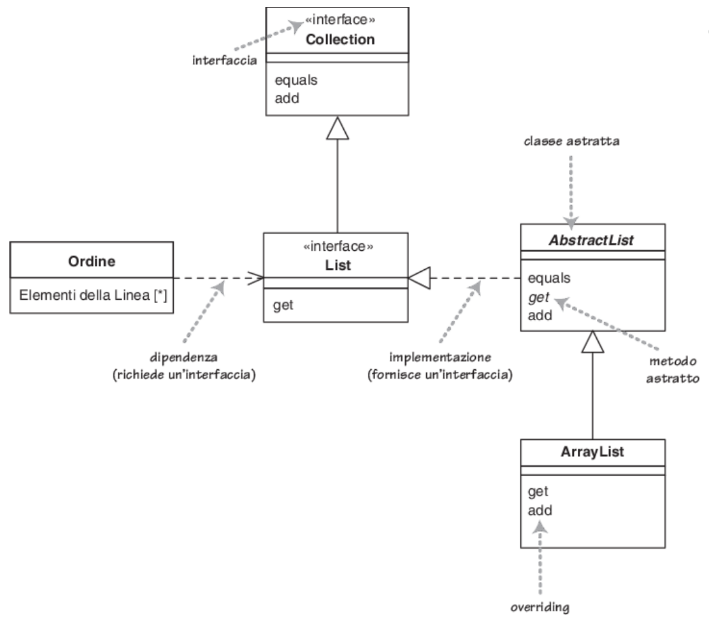
\includegraphics[width=0.5\textwidth]{figures/cl_int.png}
          \end{center}
        \end{figure}
    \subsection{Notazione Compatta Lollipop}
      \begin{itemize}
        \item \textbf{Pallina (lollipop)} rappresenta interfaccia esposta da una classe (realization); 
        \item \textbf{Semicerchio (socket)} rappresenta servizio richiesto (dipendenza).
      \end{itemize}
      \begin{figure}[h!]
        \begin{center}
          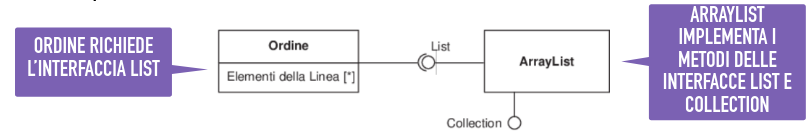
\includegraphics[width=0.5\textwidth]{figures/lollipop.png}
        \end{center}
      \end{figure}
  \section{Vincoli}
    Attraverso associazioni, molteplicità, attributi e generalizzazioni si esprimono i vincoli più importanti delle classi, UML permette la definizione di vincoli nel diagramma mediante i suoi costrutti base o mediante classi \textbf{tra parentesi graffe} in diversi linguaggi:
    \begin{itemize}
      \item linguaggio naturale; 
      \item linguaggio di programmazione;
      \item linguaggi formali specifici (OCL).
    \end{itemize}
      \begin{figure}[h!]
        \begin{center}
          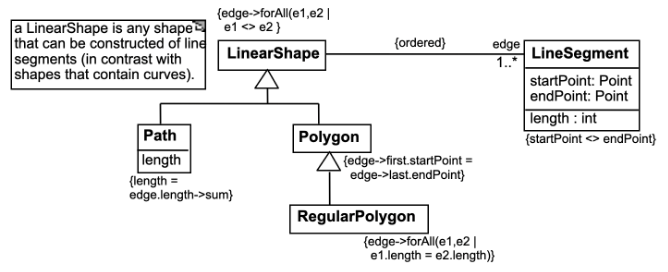
\includegraphics[width=0.5\textwidth]{figures/vin_ex.png}
        \end{center}
      \end{figure}
    \subsection{Object Constraint Language}
      Linguaggio di specifica progettato per specificare vincoli nei moduli SW, un'espessione OCL specifica un vincolo (predicato logico) sul sistema che deve assumere valore vero. Gli statements OCL sono costruiti in 3 parti:
      \begin{itemize}
        \item \textbf{Contesto} - specifica elemento del modello UML a cui si applica (classe, associazione, attributo);
        \item \textbf{Regola} - specifica tipo di vincolo, può essere invariante \textbf{inv} (deve essere sempre vero), precondizione \textbf{pre} (deve essere vero prima dell'esecuzione di un'operazione da parte della classe) o postcondizione \textbf{post};
        \item \textbf{Espressione} - definisce il vincolo
      \end{itemize}
      \subsubsection{Sintassi}
        \[
        \text{context }\langle \text{Contesto} \rangle\ \langle \text{Regola} \rangle : \langle \text{Espressione} \rangle
        \]
      \subsubsection{Vantaggi / Svantaggi}
      \begin{itemize}
        \item \textbf{Vantaggi}: notazione formale evita ambiguità del linguaggio naturale, dai vincoli formali è possibile generare automaticamente casi di test;
        \item \textbf{Svantaggi}: OCL può generare incongruenze se chi lo scrive / legge non sonosce bene OCL.
      \end{itemize}
\end{document}
